\section{Proofs}

\label{app:proofs}
\subsection{Proof of Lemma \ref{lem:2}}
\begin{proof}
We can rewrite $V_{\tau_1}(s)$ as 

\begin{align*}
    V_{\tau_1}(s) &= \E^{\tau_1}_{a\sim\mu(\cdot|s)}[r(s,a)+\gamma\E_{s'\sim p(\cdot|s,a)}[V_{\tau_1}(s')]] \\
    & \le \E^{\tau_2}_{a\sim\mu(\cdot|s)}[r(s,a)+\gamma\E_{s'\sim p(\cdot|s,a)}[V_{\tau_1}(s')]] \\
    & = \E^{\tau_2}_{a\sim\mu(\cdot|s)}[r(s,a)+\gamma\E_{s'\sim p(\cdot|s,a)}\E^{\tau_1}_{a'\sim\mu(\cdot|s')}[r(s',a')+\gamma\E_{s''\sim p(\cdot|s',a')}[V_{\tau_1}(s'')]] \\
    & \le \E^{\tau_2}_{a\sim\mu(\cdot|s)}[r(s,a)+\gamma\E_{s'\sim p(\cdot|s,a)}\E^{\tau_2}_{a'\sim\mu(\cdot|s')}[r(s',a')+\gamma\E_{s''\sim p(\cdot|s',a')}[V_{\tau_1}(s'')]] \\
    & = \E^{\tau_2}_{a\sim\mu(\cdot|s)}[r(s,a)+\gamma\E_{s'\sim p(\cdot|s,a)}\E^{\tau_2}_{a'\sim\mu(\cdot|s')}[r(s',a')+\gamma\E_{s''\sim p(\cdot|s',a')}\E^{\tau_1}_{a''\sim\mu(\cdot|s'')}[r(s'', a'')+\ldots]] \\
    \vdots \\
    &\le V_{\tau_2}(s)
\end{align*}
\end{proof}


\section{Experimental details}

\label{app:experiments}


\paragraph{Experimental details.} For the MuJoCo locomotion tasks, we average mean returns overs 10 evaluation trajectories and 10 random seeds. For the Ant Maze tasks, we average over 100 evaluation trajectories.  We standardize MuJoCo locomotion task rewards by dividing by the difference of returns of the best and worst trajectories in each dataset. Following the suggestions of the authors of the dataset, we subtract $1$ from rewards for the Ant Maze datasets. We use $\tau=0.9$ and $\beta=10.0$ for Ant Maze tasks and $\tau=0.7$ and $\beta=3.0$ for MuJoCo locomotion tasks.
We use Adam optimizer~\citep{kingma2014adam} with a learning rate $3\cdot10^{-4}$ and 2 layer MLP with ReLU activations and 256 hidden units for all networks. We use cosine schedule for the actor learning rate. We parameterize the policy as a Gaussian distribution with a state-independent standard deviation. We update the target network with soft updates with parameter $\alpha=0.005$. And following \cite{brandfonbrener2021offline} we clip exponentiated advantages to $(-\infty, 100]$. We implemented our method in the JAX~\citep{jax2018github} framework using the Flax~\citep{flax2020github} neural networks library.

{
\paragraph{Extended results on Locomotion and Ant Maze tasks.}

We present learning curves for MuJoCo locomotion tasks in \Cref{fig:curves_mujoco}.
We also present results on Locomotion and Ant Maze for different values of $\tau$ in \Cref{fig:antmaze_full} and \Cref{tab:antmaze-full}. We want to emphasize that $\tau=0.5$ corresponds to using the mean squared error instead of expectile regression.
}
\begin{figure}
    \centering
    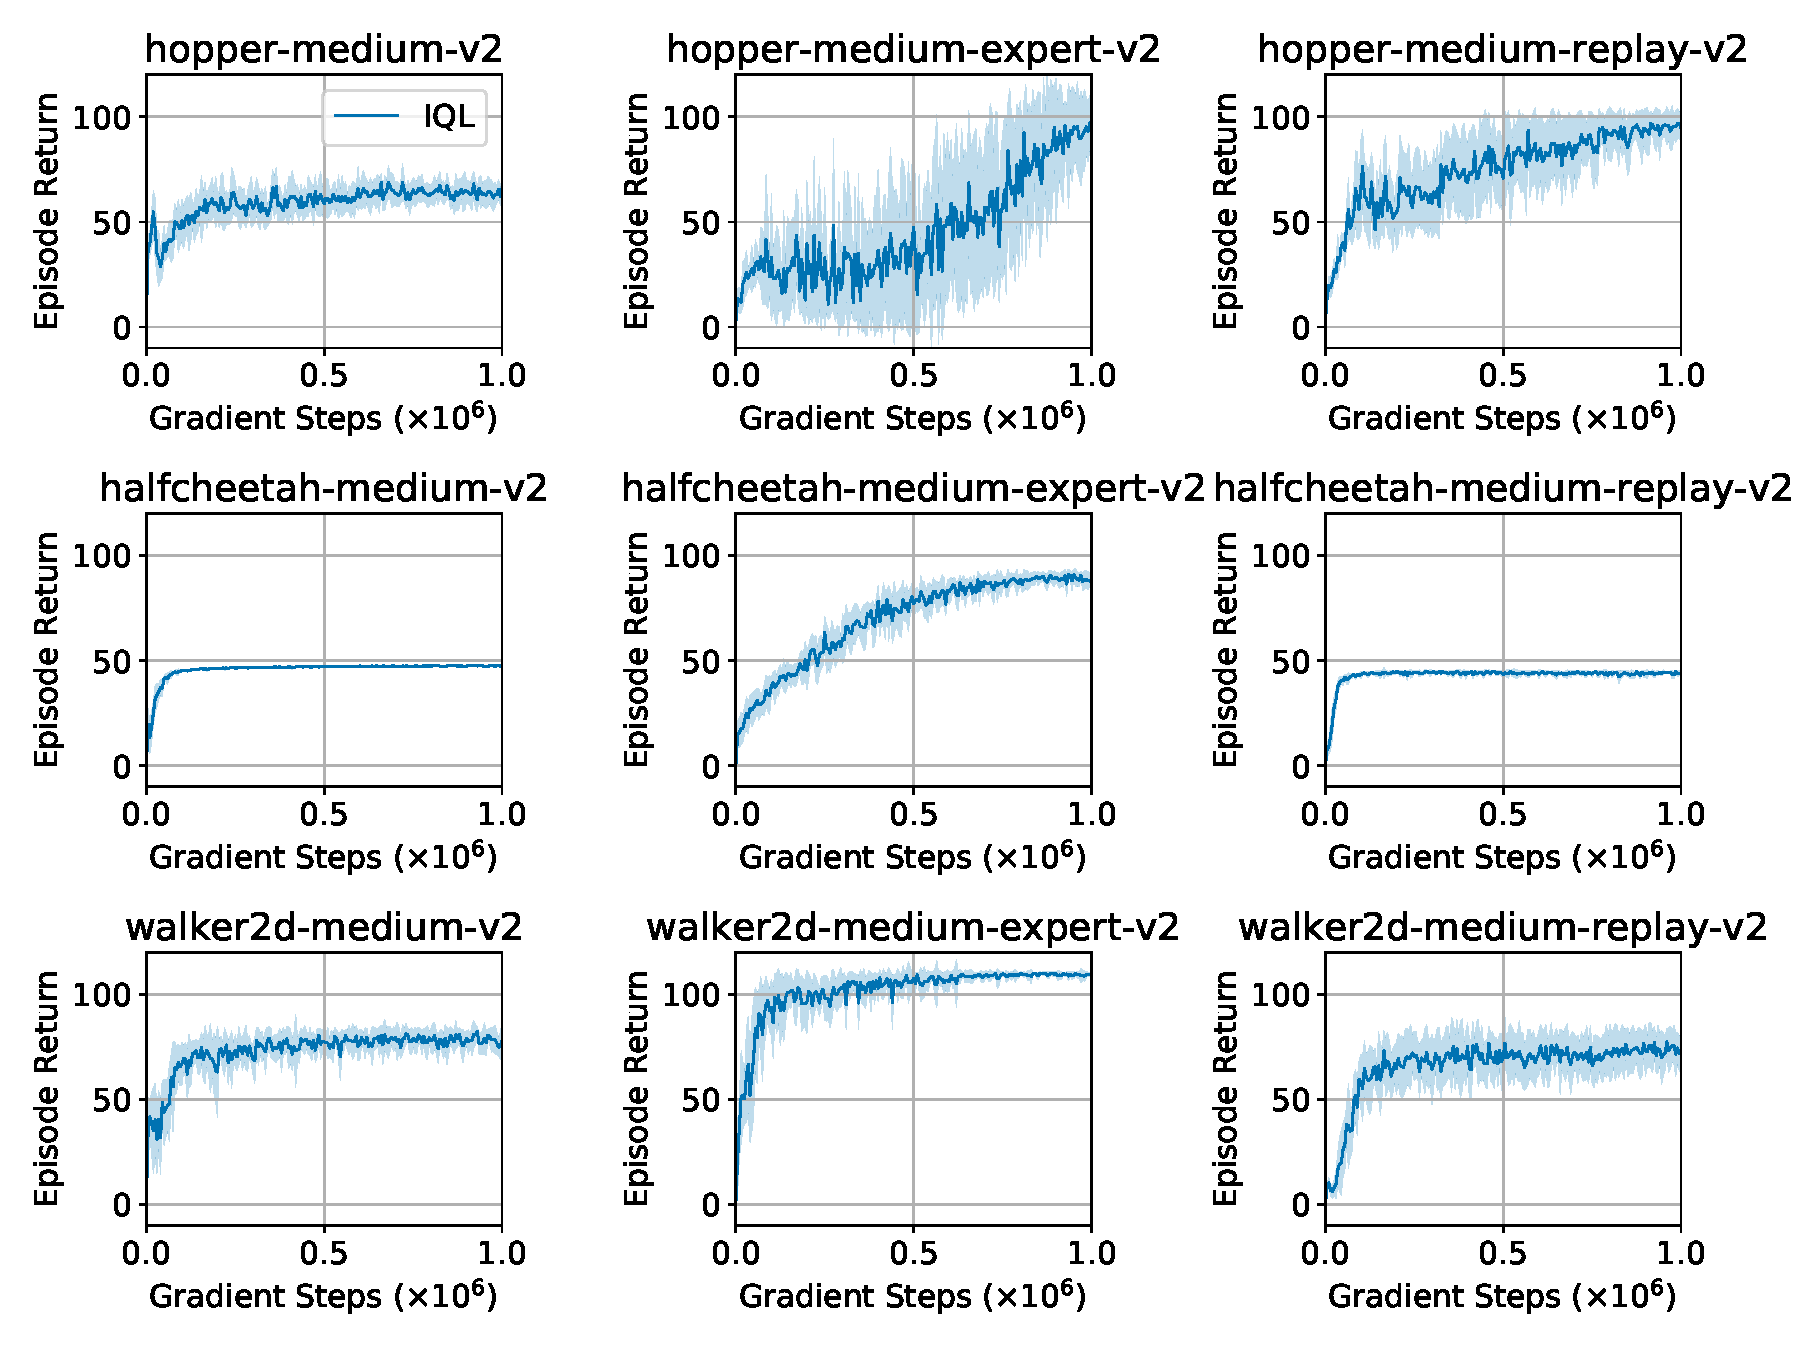
\includegraphics[width=\textwidth]{iql/images/curves_mujoco.pdf}
    \caption{Learning curves for MuJoCo locomotion tasks.}
    \label{fig:curves_mujoco}
\end{figure}

\begin{figure}
    \centering
    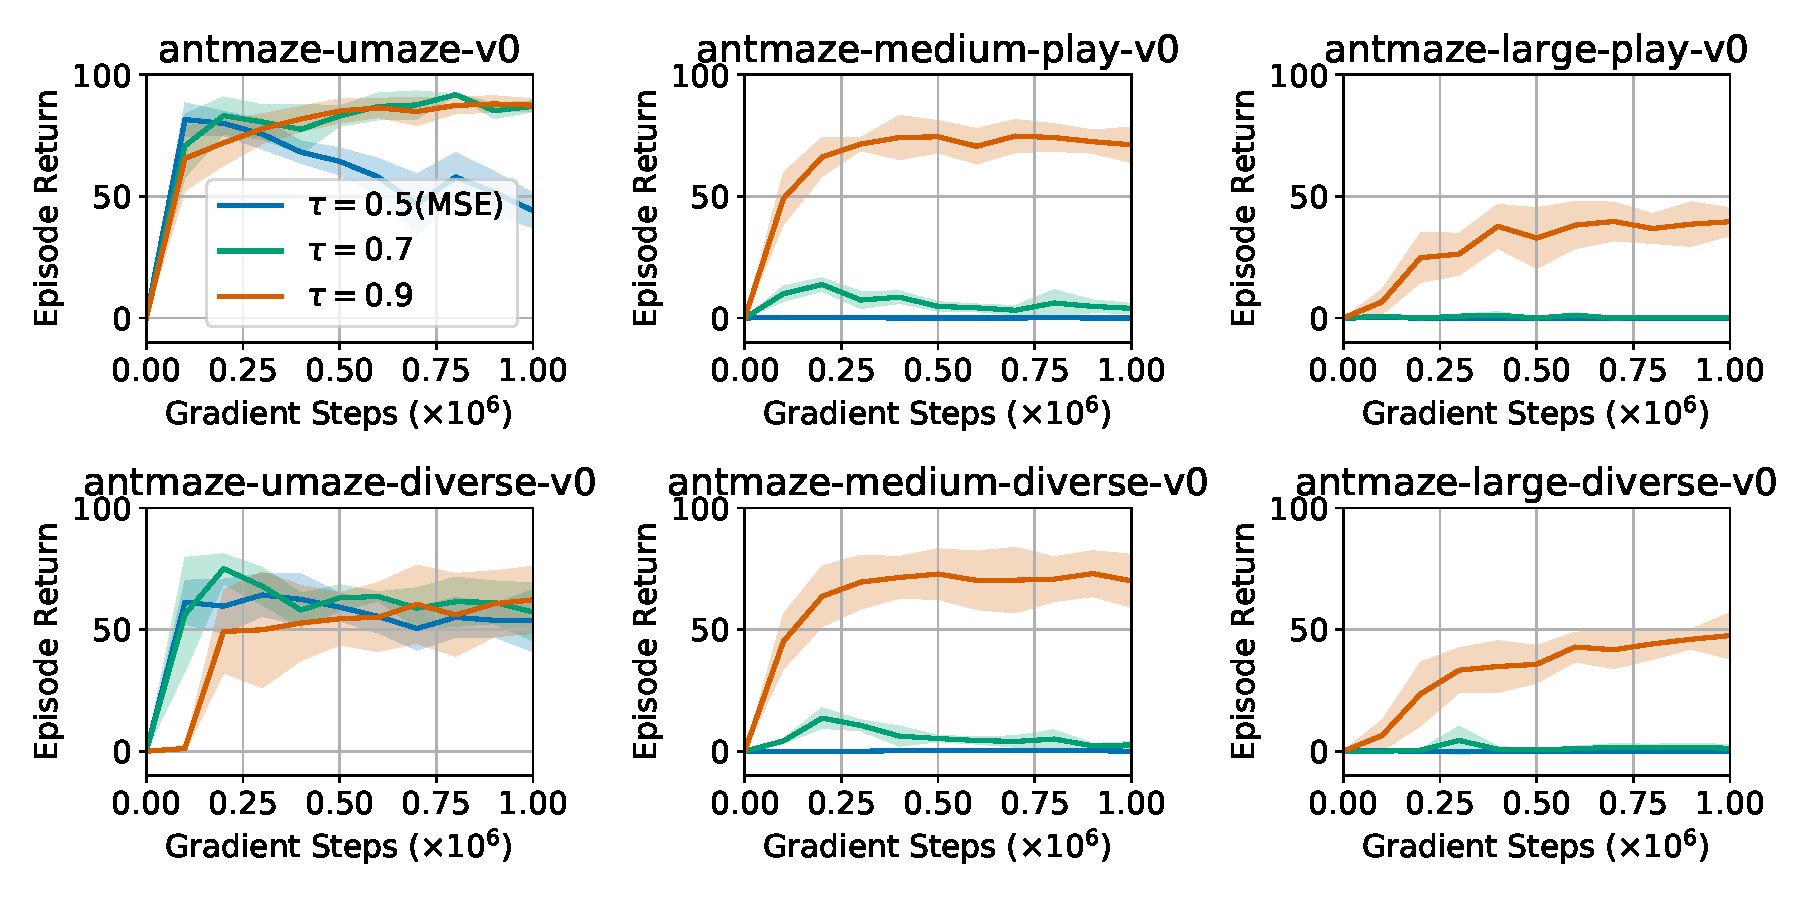
\includegraphics[width=\textwidth]{iql/images/antmaze_full.pdf}
    \caption{Results on Ant Maze for different values of $\tau$. Note that $\tau=0.5$ corresponds to using the mean squared error instead of expectile regression.}
    \label{fig:antmaze_full}
\end{figure}

\begin{table}[ht!]
\centering
\caption{Effect of $\tau$. Fitting $V(s)$ with mean squared error ($\tau=0.5$) is not sufficient to propagate the signal through recursion and fails to solve more challenging medium and large tasks.}\label{tab:antmaze-full}
\resizebox{\textwidth}{!}{
\begin{tabular}{l||rrrr}
&IQL w/ $\tau=0.5$ (MSE) &IQL w/ $\tau=0.7$ &IQL w/ $\tau=0.9$ \\\hline
antmaze-umaze-v0 &44.2$\pm$7.2 &87.0$\pm$2.3 &87.5$\pm$2.6 \\
antmaze-umaze-diverse-v0 &53.6 $\pm$12.7 &57.2$\pm$11.9 &62.2$\pm$13.8 \\
antmaze-medium-play-v0 &0.0$\pm$0.0 &4.0$\pm$2.0 &71.2 $\pm$7.3 \\
antmaze-medium-diverse-v0 &0.0 $\pm$0.0 &2.6$\pm$1.4 &70.0$\pm$10.9 \\
antmaze-large-play-v0 &0.0$\pm$0.0 &0.2$\pm$0.4 &39.6 $\pm$5.8 \\
antmaze-large-diverse-v0 &0.0 $\pm$0.0 &1.2$\pm$1.6 &47.5$\pm$9.5 \\ \hline\hline 
total &97.8$\pm$19.9 &152.2$\pm$19.6 &378.0$\pm$49.9 \\
\end{tabular}}
\end{table}

\paragraph{Results on Franca Kitchen and Adoit tasks.}
For Franca Kitchen and Adroit tasks we use $\tau=0.7$ and the inverse temperature $\beta=0.5$. Due to the size of the dataset, we also apply Dropout~\citep{srivastava2014dropout} with dropout rate of $0.1$ to regularize the policy network. See complete results in \Cref{tab:franca_adroit}.


\begin{table}[!htp]\centering
\caption{Evaluation on Franca Kitchen and Adroit tasks from D4RL}\label{tab:franca_adroit}
\resizebox{\textwidth}{!}{
\begin{tabular}{l||rrrrr|r}
dataset &BC &BRAC-p &BEAR &Onestep RL &CQL &Ours \\ \hline
kitchen-complete-v0 &\textbf{65.0} &0.0 &0.0 &- &43.8 &\textbf{62.5} \\
kitchen-partial-v0 &38.0 &0.0 &0.0 &- &\textbf{49.8} &\textbf{46.3} \\
kitchen-mixed-v0 &\textbf{51.5} &0.0 &0.0 &- &\textbf{51.0} &\textbf{51.0} \\ \hline
kitchen-v0 total &\textbf{154.5} &0.0 &0.0 &- &144.6 &\textbf{159.8} \\ \hline
pen-human-v0 &63.9 &8.1 &-1.0 &- &37.5 &\textbf{71.5} \\
hammer-human-v0 &1.2 &0.3 &0.3 &- &\textbf{4.4} &1.4 \\
door-human-v0 &2 &-0.3 &-0.3 &- &\textbf{9.9} &4.3 \\
relocate-human-v0 &0.1 &-0.3 &-0.3 &- &0.2 &0.1 \\
pen-cloned-v0 &37 &1.6 &26.5 &\textbf{60.0} &39.2 &37.3 \\
hammer-cloned-v0 &0.6 &0.3 &0.3 &\textbf{2.1} &\textbf{2.1} &\textbf{2.1} \\
door-cloned-v0 &0.0 &-0.1 &-0.1 &0.4 &0.4 &\textbf{1.6} \\
relocate-cloned-v0 &-0.3 &-0.3 &-0.3 &-0.1 &-0.1 &-0.2 \\ \hline
adroit-v0 total &104.5 &9.3 &25.1 &- &93.6 &\textbf{118.1} \\ \hline \hline
total &259 &9.3 &25.1 &- &238.2 &\textbf{277.9} \\
\end{tabular}}
\end{table}

\section{Finetuning experimental details}
\label{app:finetuning}
For finetuning experiments, we first run offline RL for 1M gradient steps. Then we continue training while collecting data actively in the environment and adding that data to the replay buffer, running 1 gradient update / environment step. All other training details are kept the same between the offline RL phase and the online RL phase. For dextrous manipulation environments~\citep{rajeswaran2018dextrous}, we use $\tau=0.8$ and $\beta=3.0$, 25000 offline training steps, and add Gaussian noise with standard deviation $\sigma=0.03$ to the policy for exploration.

\begin{table}[!htp]\centering
%\resizebox{\textwidth}{!}{
\begin{tabular}{ L{6cm} ||p{2.8cm} | p{2.8cm}  }
    \centering
    Dataset & Offline & Online \\
    % Dataset & AWAC \; Offline$\rightarrow$Online & CQL Offline $\rightarrow$ Online & Ours Offline $\rightarrow$ Online \\
    \hline
    antmaze-umaze-v0 & 70.1  $\rightarrow$ \textbf{99.4} & \textbf{86.7}  $\rightarrow$ \textbf{96.0} \\
    antmaze-umaze-diverse-v0 & 31.1  $\rightarrow$ \textbf{99.4} & \textbf{75.0}  $\rightarrow$ 84.0 \\
    antmaze-medium-play-v0 & 23.0  $\rightarrow$ 0.0 & \textbf{72.0}  $\rightarrow$ \textbf{95.0} \\
    antmaze-medium-diverse-v0 & 23.0  $\rightarrow$ 32.3 & \textbf{68.3}  $\rightarrow$ \textbf{92.0} \\
    antmaze-large-play-v0 & 1.0  $\rightarrow$ 0.0 & \textbf{25.5}  $\rightarrow$ \textbf{46.0} \\
    antmaze-large-diverse-v0 & 1.0  $\rightarrow$ 0.0 & \textbf{42.6}  $\rightarrow$ \textbf{60.7} \\ \hline
    % antmaze-v0 total & 151.5 $\rightarrow$ 231.1 & \textbf{370.1} $\rightarrow$ \textbf{473.7} \\ \hline
    pen-binary-v0 & 46.2 $\pm$ 6.3 & 63.3  $\pm$ 1.9 \\
    door-binary-v0 & 1.3  $\pm$ 0.7 & 42.0  $\pm$ 3.2 \\
    relocate-binary-v0 & 0.3  $\pm$ 0.4 & 23.3  $\pm$ 14.5 \\ \hline
    % hand-v0 total & 31.5 \; $\rightarrow$ 9.9 & 38.1 \; $\rightarrow$ \textbf{124.0} \\ \hline \hline
    % total & 182.8 $\rightarrow$ 241.0 & \textbf{408.2} $\rightarrow$ \textbf{597.7}
    %%SL.10.3: why is CQL offline ant maze much worse here than it is in Table 1? is that a bug?
\end{tabular}
%}
\caption{Error bars for fine-tuning experiments with 20 seeds, showing one standard deviation.}
\label{tab:finetuning}
\end{table}


For baselines we compare to the original implementations of AWAC~\citep{nair2020awac} and CQL~\citep{kumar2020conservative}. For AWAC we used \url{https://github.com/rail-berkeley/rlkit/tree/master/rlkit}. We found AWAC to overfit heavily with too many offline gradient steps, and instead used 25000 offline gradient steps as in the original paper. For the dextrous manipulation results, we report average return normalized from 0 to 100 for consistency, instead of success rate at the final timestep, as reported in~\citet{nair2020awac}. For CQL, we used \url{https://github.com/aviralkumar2907/CQL}. Our reproduced results offline are worse than the reported results, particularly on medium and large antmaze environments. We were not able to improve these results after checking for discrepancies with the CQL paper authors and running CQL with an alternative implementation (\url{https://github.com/tensorflow/agents}). Thus, although for offline experiments (Table~\ref{tab:d4rl}) we report results from the original paper, for finetuning experiments we did not have this option and report our own results running CQL in Table~\ref{tab:finetuning}.

\section{Connections to prior work}
In this section, we discuss how our approach is related to prior work on offline reinforcement learning. In particular, we discuss connections to BCQ~\cite{fujimoto2019off}.
%, Onestep RL~\cite{brandfonbrener2021offline} and AWAC~\cite{nair2020awac}.

Our batch constrained optimization objective is similar to BCQ~\citep{fujimoto2019off}. In particular, the authors of BCQ build on the Q-learning framework and define the policy as
\begin{equation}
\label{eqn:bcq_policy}
\pi(s) = \argmax_{\substack{a\\s.t.(s, a)\in \D}}Q(s,a).
\end{equation}
Note that in contrast to the standard Q-learning, maximization in \Cref{eqn:bcq_policy} is performed only over the state-action pairs that appear in the dataset. In \cite{fujimoto2019off}, these constraints are implemented via fitting a generative model $\mu(\cdot|s)$ on the dataset, sampling several candidate actions from this generative model, and taking an argmax over these actions:
$$
\pi(s) = \argmax_{\{a_i| a_i \sim \mu(\cdot|s), i=1\ldots N\}}Q(s,a_i).
$$
However, this generative model can still produce out-of-dataset actions that will lead to querying undefined Q-values. Thus, our work introduces an alternative way to optimize this objective without requiring an additional density model. Our approach avoids this issue by enforcing the hard constraints via estimating expectiles. Also, it is worth mentioning that a number of sampled actions $N$ in BCQ has similar properties to choosing a particular expectile $\tau$ in our approach.


Note that our algorithm for optimal value approximation does not require an explicit policy, in contrast to other algorithms for offline reinforcement learning for continuous action spaces~\citep{fujimoto2019off, fujimoto2021minimalist, wu2019behavior, kostrikov2021offline, kumar2019stabilizing, kumar2020conservative}. Thus, we do not need to alternate between actor and critic updates, though with continuous actions, we must still extract an actor at the end once the critic converges.

\section{Different Estimators of $V(s)$}

{
We also evaluate different ways to estimate the value function $V(s)$ (\Cref{tab:abm}). We compare $V(s)$ learned with expectile regression as in IQL with $V(s)$ estimated with several samples from the learned policy as in ABM~\citep{siegel2020keep}. In particular, we use $N=20$ to estimate the value function.}


\begin{table}[!htp]\centering
\caption{Different estimators of $V(s)$}\label{tab:abm}
%\scriptsize
\begin{tabular}{L{7cm}|rrr}
& IQL & $V(s)=\sum_{i=1}^N Q(s,a_i) / N$ \\\hline
hopper-medium-v2 &66.2$\pm$5.7 &69.5$\pm$3.9 \\
hopper-medium-expert-v2 &91.5$\pm$14.3 &75.8$\pm$37.8 \\
hopper-medium-replay-v2 &94.7$\pm$8.6 &64.7$\pm$22.6 \\
halfcheetah-medium-v2 &47.4$\pm$0.2 &47.2$\pm$0.2 \\
halfcheetah-medium-expert-v2 &86.7$\pm$5.3 &93.0$\pm$0.9 \\
halfcheetah-medium-replay-v2 &44.2$\pm$1.2 &45.1$\pm$0.3 \\
walker2d-medium-v2 &78.3$\pm$8.7 &72.0$\pm$24.6 \\
walker2d-medium-expert-v2 &109.6$\pm$1.0 &110.7$\pm$0.4 \\
walker2d-medium-replay-v2 &73.8$\pm$7.1 &83.3$\pm$3.0 \\ \hline
locomotion total &692.4$\pm$52.1 &661.4$\pm$93.7 \\ \hline
antmaze-umaze-v0 &87.5$\pm$2.6 &96.4$\pm$1.8 \\
antmaze-medium-play-v0 &71.2$\pm$7.3 &0.0$\pm$0.0 \\
antmaze-large-play-v0 &39.6$\pm$5.8 &0.0$\pm$0.0 \\
antmaze-umaze-diverse-v0 &62.2$\pm$13.8 &57.5$\pm$6.3 \\
antmaze-medium-diverse-v0 &70.0$\pm$10.9 &0.0$\pm$0.0 \\
antmaze-large-diverse-v0 &47.5$\pm$9.5 &0.0$\pm$0.0 \\ \hline
antmaze total &378.0$\pm$49.9 &153.9$\pm$8.1 \\
\end{tabular}
\end{table}
%\end{document}
